\documentclass[conference]{IEEEtran}
\IEEEoverridecommandlockouts
% The preceding line is only needed to identify funding in the first footnote. If that is unneeded, please comment it out.
\usepackage{cite}
\usepackage{amsmath,amssymb,amsfonts}
\usepackage{algorithmic}
\usepackage{graphicx}
\usepackage{textcomp}
\usepackage{xcolor}
\def\BibTeX{{\rm B\kern-.05em{\sc i\kern-.025em b}\kern-.08em
    T\kern-.1667em\lower.7ex\hbox{E}\kern-.125emX}}
\begin{document}

\title{Impact of network topology in collaborative learning dynamics}

\begin{center}
\author{
\IEEEauthorblockN{Kamla Singh}
\IEEEauthorblockA{\textit{M.Sc. (Economics)} \\
\textit{Department of Humanities and Social Sciences}\\
\textit{Indian Institute of Technology Roorkee}\\
Roorkee, India \\
kamla\_s@hs.iitr.ac.in}
\and
\IEEEauthorblockN{Abhishek Samantray}
\IEEEauthorblockA{\textit{Assistant Professor} \\
\textit{Department of Humanities and Social Sciences}\\
\textit{Indian Institute of Technology Roorkee}\\
Roorkee, India \\
abhishek.samantray@hs.iitr.ac.in}
}
\end{center}

\maketitle

\begin{abstract}
This project investigates the impact of network topology on collective learning, focusing on how various network structures influence the discovery and sharing of knowledge within a networked group of agents. In many collaborative environments—from scientific research to technological innovation—the network structure that connects agents can profoundly impact the quality and speed of collective learning outcomes. This study is motivated by recent empirical findings showing that efficient communication networks can quickly disseminate information, they may also restrict innovation by causing premature convergence on suboptimal solutions.

Through simulations of both efficient and inefficient network configurations, this project examines how the efficiency and structure of communication pathways affect agents’ capacity to explore and exploit solutions within a complex problem landscape. We aim to uncover the trade-offs between solution speed and diversity by analyzing learning outcomes in both fully connected and sparsely connected lattice networks. The findings contribute to a deeper understanding of network design principles that can optimize collective learning, offering potential applications in organizational management, research collaborations, and AI systems that rely on distributed knowledge acquisition.

\end{abstract}


\section{Introduction}
In complex problem-solving environments, network structure plays a crucial role in shaping how information is shared and how solutions are collectively discovered. Traditional theories in organizational and communication sciences suggest that tightly connected, efficient networks—characterized by short path lengths and rapid information diffusion—enable faster solution convergence. In these networks, agents can quickly exchange information, allowing groups to reach consensus on solutions at an accelerated pace. Fields such as engineering, medicine, and data science have embraced this model, aiming to enhance productivity and learning outcomes through highly efficient communication structures.

However, recent research has challenged this perspective, proposing that efficient communication networks may inadvertently stifle innovation. Studies suggest that when agents in a network are closely connected, they may settle on readily available solutions rather than exploring alternative possibilities. This phenomenon is particularly relevant in contexts where problem landscapes are complex and rugged, containing multiple local optima that may not lead to the best possible solutions. In such settings, fast information diffusion may hinder the discovery of novel solutions, as agents quickly converge on familiar options rather than persist in exploratory behaviors. This alternative perspective implies that a certain degree of inefficiency—or structural "slowness"—in a network can be beneficial, as it fosters diverse solution pathways and sustains exploration over exploitation.

This project builds on these competing theories by investigating how variations in network topology affect collective learning outcomes. Specifically, we simulate two types of network structures: a fully connected, efficient network where agents have immediate access to each other's solutions and a lattice-based, inefficient network where each agent is connected to a limited number of neighbors. In the fully connected network, information flows freely and quickly, which we hypothesize will lead to faster but potentially narrower learning outcomes. Conversely, the lattice network’s limited connectivity promotes more isolated exploration among clusters of agents, potentially enabling a broader diversity of solutions over time. By analyzing the quality and speed of solutions generated within each network, this study seeks to provide a nuanced understanding of the relationship between network structure and collective learning.

Understanding the optimal balance between network efficiency and solution diversity has significant implications. In organizational settings, managers could adjust team structures to either prioritize quick consensus or support more innovative, exploratory work. Additionally, in AI systems or agent-based simulations where collective intelligence is needed to solve complex problems, our findings may inform the design of interaction protocols that balance rapid information sharing with exploratory potential. Ultimately, this study aims to contribute actionable insights into how networked systems can be structured to maximize collective knowledge acquisition.

\section{Background}

\subsection{Network topology}

In this study, we explore two distinct network topologies that represent contrasting modes of information diffusion and agent interaction: the Efficient Network and the Inefficient Network.

\begin{itemize}
    \item \textbf{Efficient Network (Fully Connected):} The efficient network configuration consists of a fully connected topology, where each agent is linked to every other agent in the system. This structure maximizes connectivity, enabling immediate and unrestricted exchange of information among all agents. The high degree of connectivity is anticipated to accelerate convergence, as agents can swiftly adopt any superior solutions identified within the network. However, the rapid dissemination of information may also introduce risks of premature convergence, potentially locking the system into suboptimal equilibria before a thorough exploration of the problem space is achieved. This topology is expected to favor exploitation over exploration, prioritizing quick consensus at the potential cost of innovation.
    \item \textbf{Inefficient Network:} The inefficient network is designed as a sparse one-dimensional lattice, where each agent is connected only to a limited number of immediate neighbors. This topology restricts the flow of information, slowing down the spread of discovered solutions across the network. The localized interactions foster a more decentralized learning process, allowing agents to explore diverse regions of the problem landscape independently. The slower rate of information diffusion in this structure is hypothesized to enhance the overall diversity of solutions, as agents are less influenced by the discoveries of distant peers. This configuration is expected to strike a balance between exploration and exploitation, potentially leading to more robust, innovative solutions as agents navigate a rugged fitness landscape.
\end{itemize}


\section{Agent Behavior and Decision-Making Process}

In general, agents operating within a networked environment must navigate the trade-off between exploration and exploitation, two fundamental strategies for decision-making in adaptive systems, organizational learning, and problem-solving tasks:

\begin{itemize}
    \item \textbf{Exploration:} Exploration refers to the process by which agents seek out new information, test novel approaches, or experiment with alternative solutions. This behavior is driven by the need to gather knowledge about the environment or problem space, often involving incremental changes to current strategies. Exploration is typically characterized by a high level of uncertainty, as agents pursue options that may not yield immediate rewards but hold the potential for discovering superior solutions in the long run. It encourages diversity in strategies and solutions, as agents independently test different paths rather than converging prematurely on a shared outcome.
    \item \textbf{Exploitation:} Exploitation involves agents utilizing known information to maximize immediate gains. Instead of seeking out new alternatives, agents focus on leveraging existing knowledge, adopting strategies or solutions that have been identified as successful. Exploitation allows for efficient use of resources, as agents capitalize on the best available solutions rather than investing time in uncertain explorations. This behavior often leads to faster convergence on a solution but may risk overlooking potentially better alternatives that have not yet been explored.
\end{itemize}

In adaptive systems, finding an optimal balance between exploration and exploitation is crucial. A strong focus on exploration can lead to high innovation and discovery of novel solutions but may also incur higher costs and slower convergence. Conversely, excessive exploitation can result in rapid optimization but at the risk of stagnation or local optima, where the system settles on suboptimal solutions due to insufficient exploration.

The balance between these strategies is influenced by various factors, including the nature of the problem landscape, the structure of the network, and the goals of the agents. In dynamic and uncertain environments, greater emphasis on exploration may be beneficial to adapt to changes, while in stable and well-understood contexts, exploitation may yield better results. Successful decision-making processes often employ adaptive mechanisms that adjust the balance between exploration and exploitation based on feedback and evolving conditions within the system.

\subsection{Network Performance Metrics}

The performance of the agents within each network configuration is evaluated based on two key metrics: Best Solution Quality and Average Solution Quality. These metrics are derived from the Bayesian Information Criterion (BIC), which is used to assess the quality of solutions obtained by the agents in solving the linear regression problem. The BIC is particularly suitable for this context as it penalizes the complexity of the model, preventing overfitting while rewarding better model fits.

\begin{itemize}
    \item \textbf{Bayesian Information Criterion (BIC):}
The BIC is a widely used statistical criterion for model selection that provides a trade-off between the goodness of fit and the complexity of the model. For a given set of data and a model, the BIC is defined as:

\begin{equation}
\text{BIC} = \ln(n)k - 2\ln(\hat{L})
\end{equation}
Where:
\begin{itemize}
    \item $n$ is the number of data points,
    \item $k$ is the number of parameters in the model,
    \item $\hat{L}$ is the maximum value of the likelihood function.
\end{itemize}

For linear regression, it can be expressed as
\begin{equation}
\text{BIC} = n \ln\left(\frac{\sum_{i=1}^{n} (y_i - \hat{y}_i)^2}{n}\right) + k \ln(n)
\end{equation}
Where:
\begin{itemize}
    \item $n$ is the number of data points,
    \item $k$ is the number of parameters (including the intercept),
    \item $y_i$ are the observed values,
    \item $\hat{y}_i$ are the predicted values from the regression model.
\end{itemize}

In our model, the agents are solving a linear regression problem, and the BIC is used to evaluate the quality of the coefficients they determine. A lower BIC indicates a better model with a good balance between fitting the data and avoiding unnecessary complexity. In other words, a solution with a lower BIC corresponds to a regression model that explains the data well while using fewer parameters, thereby avoiding overfitting.

\item \textbf{}{Best Solution Quality:} 
The Best Solution Quality refers to the lowest BIC score achieved by any agent in the network over the course of the simulation. This metric is particularly important as it reflects the network's ability to support the discovery of high-quality solutions. In a networked environment, the diffusion of information and the strategies employed by agents (exploration and exploitation) can lead to the identification of the optimal or near-optimal solutions.

A lower BIC in the best solution indicates that at least one agent has managed to find a regression model that is both highly accurate and efficient, suggesting that the network is capable of reaching good solutions despite the challenges posed by a rugged fitness landscape. The best solution also provides insight into the effectiveness of the collective learning process in the network, as it shows whether the agents, given their connectivity structure, are able to converge toward an optimal or near-optimal model.

\item \textbf{Average Solution Quality:}
The Average Solution Quality is the mean BIC score across all agents in the network at the end of the simulation. This metric offers a broader perspective on the overall performance of the network, capturing the typical solution quality that emerges across all agents. A lower average BIC indicates that, on average, the agents have converged on solutions that are of higher quality, suggesting efficient knowledge diffusion and learning within the network.

The average BIC score also serves as an indicator of the learning efficiency within the network. In a highly connected network, agents are likely to converge more quickly to a shared solution, which may lead to a lower average BIC. In contrast, in a sparsely connected network, the average BIC might be higher due to slower information diffusion and a greater degree of local exploration. Thus, this metric provides valuable insight into how the structure of the network impacts the overall learning process and the ability of agents to collectively approach an optimal solution.

\end{itemize}

The use of the BIC in evaluating solution quality is particularly well-suited for this type of agent-based model, where the goal is to solve a complex, multi-dimensional problem. The BIC encourages agents to find solutions that are not only accurate but also generalizable, avoiding overfitting to local features of the data. In the context of the simulation, BIC serves as both a measure of solution quality and a guide for agent decision-making. By minimizing BIC, agents improve both the fit of their models and the efficiency of the learning process, making it an essential performance metric in this study.

Ultimately, the comparison of the best and average BIC scores across different network configurations allows us to assess the effects of network structure on collective learning dynamics, highlighting the balance between exploration, exploitation, and information diffusion.

\section{Methodology}

In this study, we employ a simulation-based approach to examine how different network structures influence collective learning dynamics and the trade-off between exploration and exploitation in a complex problem landscape. The simulation setup involves two distinct network configurations: an Efficient Network and an Inefficient Network, each consisting of $N$ nodes. These nodes function as agents tasked with solving a linear regression problem, navigating a rugged fitness landscape characterized by multiple local optima. The quality of each solution is assessed using the Bayesian Information Criterion (BIC), a metric that accounts for both model fit and complexity.

\subsection{Network Configuration and Agent Interaction}
The Efficient Network is modeled as a fully connected graph, where every agent has direct access to all other agents in the network. This high degree of connectivity facilitates rapid information exchange, enabling agents to quickly adopt superior solutions discovered by any member of the network. In contrast, the Inefficient Network is structured as a sparse one-dimensional lattice, where each agent is connected to a limited number of nearest neighbors, represented by $D$ , the average degree of a node. This limited connectivity slows the diffusion of information, encouraging more localized learning and reducing the risk of premature convergence on suboptimal solutions.

\subsection{Decision-Making Process: Exploration vs. Exploitation}
During each round of the simulation, agents must choose between two decision-making strategies: exploration and exploitation. This choice reflects the inherent trade-off between seeking new solutions independently and leveraging the successful discoveries of others. In our model, the probability of choosing exploitation is directly proportional to the number of neighbors an agent has. This means that agents in more densely connected networks (e.g., the efficient network) are more inclined to exploit, while those in sparsely connected networks (e.g., the inefficient lattice) are more likely to explore.

\textbf{Exploration: }
In the exploration phase, an agent attempts to enhance its own solution by making small, incremental adjustments to the coefficients of the regression model. This is implemented using partial regression, where a single parameter is modified, and the resulting change in the BIC score is evaluated. Exploration is a local search process, allowing agents to independently investigate new possibilities without the influence of external solutions.

\textbf{Exploitation: }
In the exploitation phase, an agent selects one of its connected neighbors and adopts its solution if it offers a lower BIC score, indicating better performance. The likelihood of an agent engaging in exploitation increases with the number of neighbors it has, reflecting the greater availability of potentially superior solutions in more connected networks. In the efficient network, this behavior leads to rapid diffusion of optimal solutions across the entire network, while in the inefficient network, exploitation remains confined to local clusters, allowing for more diverse exploration across the network.

\subsection{Simulation Procedure}
The simulation begins with the initialization of both network configurations, where each agent is assigned a random initial solution for the linear regression problem. The process unfolds over $R$ iterative rounds, during which each agent evaluates its current strategy based on its connectivity:

\begin{itemize}
    \item \textbf{Initialization: } Randomly assign initial regression coefficients to each agent and calculate the initial BIC scores.
    \item \textbf{Decision Phase: } In each round, agents determine whether to explore or exploit based on their number of neighbors. The probability of selecting exploitation is higher for agents with more neighbors, emphasizing the influence of network connectivity on decision-making.
    \item \textbf{Exploration or Exploitation: } If an agent chooses to explore, it updates one of its regression coefficients using partial regression and evaluates the change in BIC score.
    If an agent chooses to exploit, it compares its solution with that of a randomly selected neighbor. If the neighbor’s solution yields a lower BIC score, the agent adopts it.
    \item \textbf{Performance Evaluation: } After completing all $R$ rounds, we evaluate the performance of each network configuration using two primary metrics:
    Best Solution Quality: The lowest BIC score achieved by any agent, indicating the network’s capacity for discovering high-quality solutions. \\
    Average Solution Quality: The mean BIC score across all agents, reflecting the overall efficiency of knowledge diffusion and collective learning.
\end{itemize}



\subsection{Analysis}
By comparing the best and average solution quality across the efficient and inefficient networks, we can assess how network structure and connectivity influence the balance between exploration and exploitation. The dependency of exploitation probability on the number of neighbors provides a realistic representation of decision-making in networked systems, where agents in more connected environments are more inclined to capitalize on shared knowledge, while those in less connected environments maintain a higher focus on independent discovery. This analysis aims to provide insights into optimizing network design for complex, multi-dimensional problem-solving tasks

\section{Results and Discussion}

In this section, we present the results of our simulation, where the two network configurations—Efficient Network and Inefficient Network—were compared based on the performance of agents solving a linear regression problem using Bayesian Information Criterion (BIC) as the evaluation metric. The simulation was conducted with $N = 20$ agents (nodes), $D = 4$ neighbors per agent in the inefficient network, and $R = 16$ rounds of interaction. The goal was to assess the best and average solution quality in both network configurations as the simulation progressed.

\subsection{Initial Performance Differences}
At the beginning of the simulation, agents in the Efficient Network (high connectivity) achieved lower BIC scores, indicating better model fit and simplicity compared to those in the Inefficient Network (sparse connectivity). This initial gap is due to the Efficient Network’s higher degree of connectivity, which facilitated faster dissemination of superior solutions. As a result, agents in the Efficient Network could exploit high-quality solutions from their neighbors early on, rapidly improving their overall performance.

\subsection{Convergence Over Rounds}
As the simulation advanced through successive rounds, agents in the Inefficient Network exhibited substantial improvement in their BIC scores. By round 8, agents in the Inefficient Network began closing the gap in average BIC compared to those in the Efficient Network. This convergence trend continued, with the Inefficient Network approaching the Efficient Network’s solution quality by the end of the 16 rounds. The improvement was driven by gradual knowledge sharing through the exploration and exploitation phases, allowing agents in the Inefficient Network to refine their solutions despite limited connectivity.

\subsection{Best and Average Solution Quality}
In terms of best solution quality, the Efficient Network maintained a slight advantage, with the lowest BIC consistently achieved in this configuration. However, the Inefficient Network's best solutions gradually improved, reducing the difference between the two networks by the final rounds. For average solution quality, the Efficient Network initially outperformed the Inefficient Network, but by round 16, the average BIC scores in both configurations were nearly indistinguishable.

The simulation results demonstrate that while network efficiency impacts early performance, both efficient and inefficient networks can achieve similar solution quality over time given sufficient rounds of interaction. This suggests that, in collaborative settings, even sparsely connected networks can approach the performance of more connected ones through iterative exploration and exploitation.

\section{Conclusion}

In this study, we examined the impact of network connectivity on collaborative learning across diverse datasets, including Red Wine Quality, White Wine Quality, Online News Popularity, and Daily Demand Forecasting Orders. The findings reveal that initial performance disparities between inefficient (sparsely connected) and efficient (densely connected) networks were significant, with the former exhibiting higher Bayesian Information Criterion (BIC) scores, indicative of poorer model performance. This outcome was attributed to limited connectivity, which hindered effective knowledge sharing among nodes in inefficient networks.

However, as the learning process unfolded over multiple rounds, nodes in sparsely connected networks demonstrated substantial improvement, achieving BIC scores comparable to those in well-connected networks. This convergence highlights the capacity of iterative collaborative mechanisms, wherein nodes alternate between self-exploration and selective exploitation of neighbors’ solutions, to overcome the limitations imposed by reduced connectivity. Notably, the consistent patterns observed across all datasets underscore the robustness of this finding.

Overall, these results suggest that while high connectivity accelerates the initial phase of collective learning, even networks with constrained connectivity can, through iterative collaboration, converge toward high-quality solutions. This insight underscores the potential of distributed learning frameworks to adapt and thrive in scenarios with limited connectivity, offering valuable implications for the design of resilient collaborative learning systems in decentralized environments.

\subsection{Figures and Tables}

\begin{table}[htbp]
\caption{Description of the data sets $^{\mathrm{*}}$}
\begin{center}
\begin{tabular}{|l|l|l|}
\hline
\textbf{Dataset} & \textbf{Variables} & \textbf{Observations} \\
\hline
Red Wine Quality & 11 & 1599 \\
\hline
White Wine Quality & 11 & 4898 \\
\hline
Online News Popularity & 58 & 39644 \\
\hline
Daily Demand Forecasting Orders & 12 & 60 \\
\hline
\multicolumn{3}{l}{$^{\mathrm{*}}$Taken from UCI Machine Learning Repository.}
\end{tabular}
\label{tab1}
\end{center}
\end{table}

\begin{figure}[htbp]
\centerline{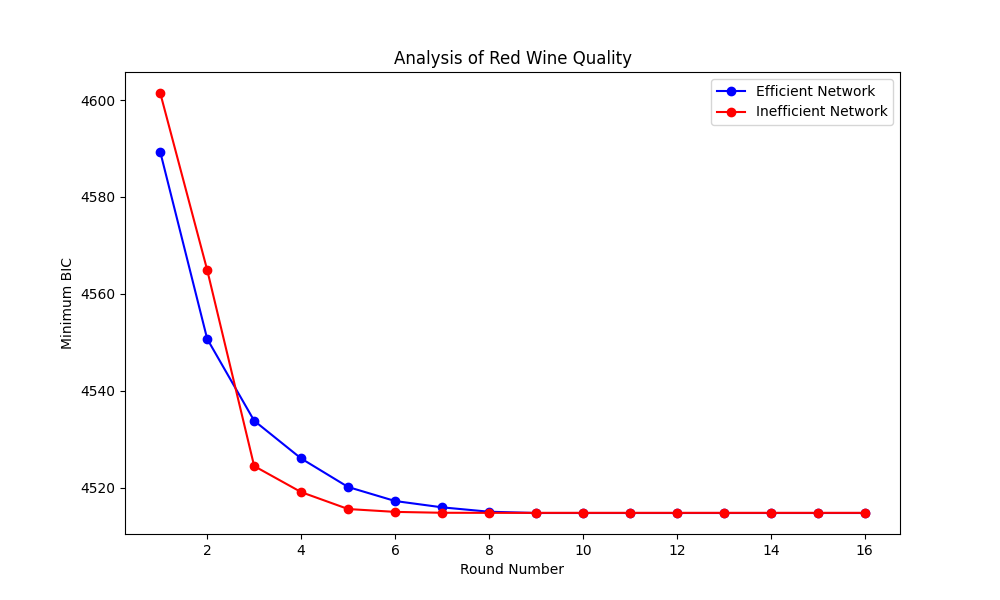
\includegraphics[scale=0.4]{figures/Red Wine Quality Min.png}}
\centerline{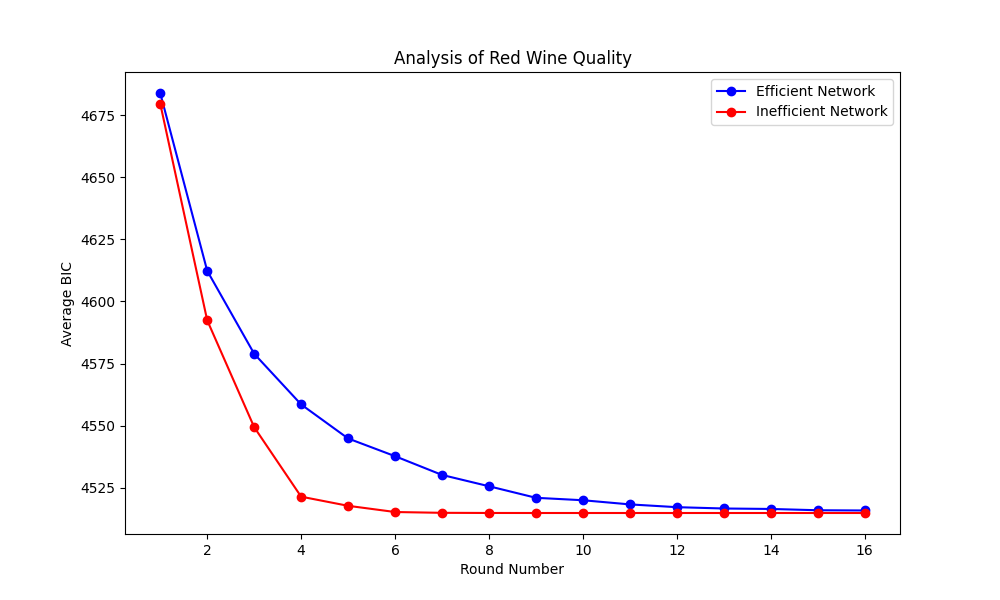
\includegraphics[scale=0.4]{figures/Red Wine Quality Avg.png}}
\caption{Red Wine Quality}
\label{fig}
\end{figure}

\begin{figure}[htbp]
\centerline{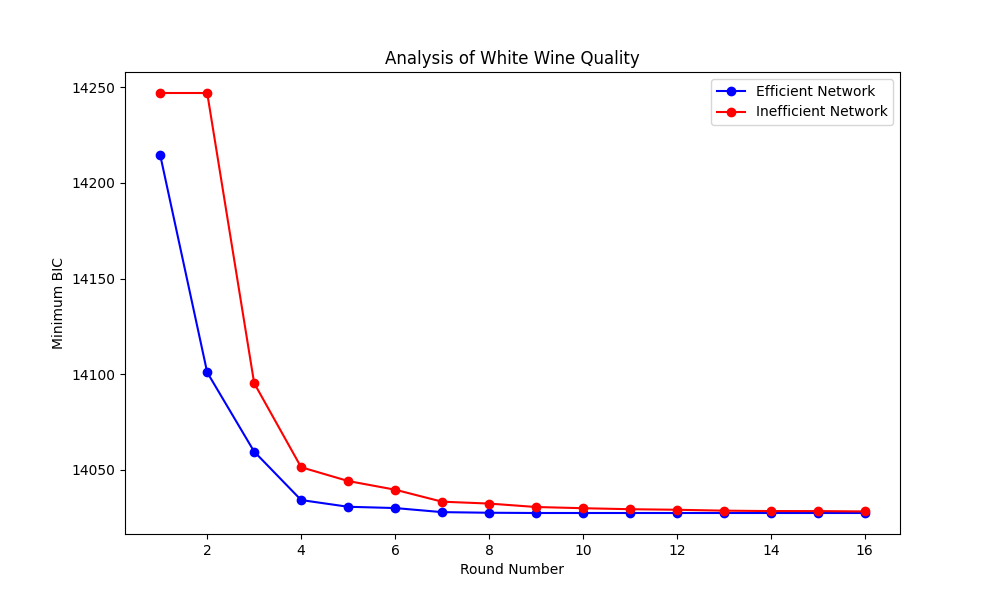
\includegraphics[scale=0.4]{figures/White Wine Quality Min.png}}
\centerline{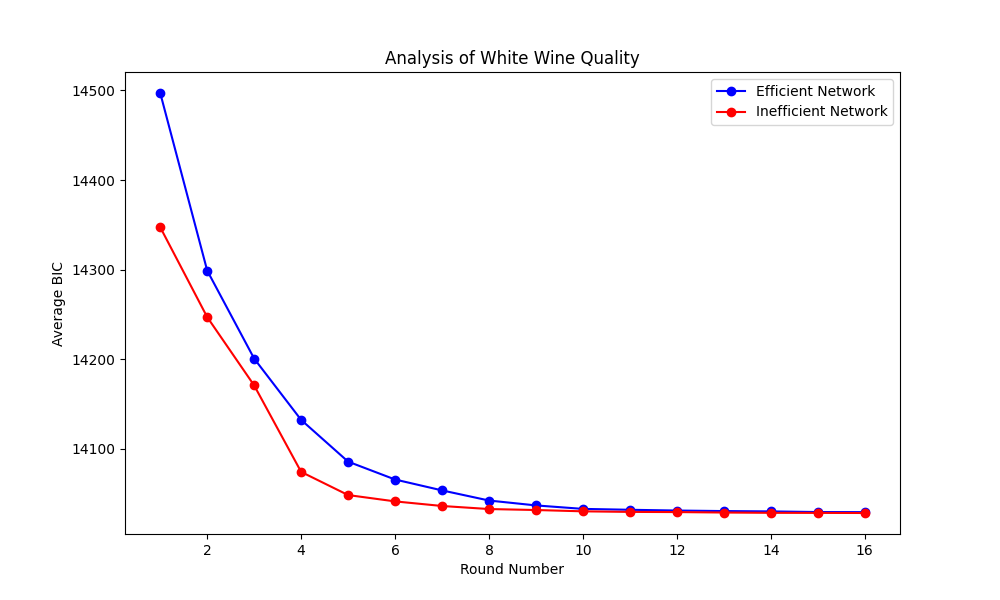
\includegraphics[scale=0.4]{figures/White Wine Quality Avg.png}}
\caption{White Wine Quality}
\label{fig}
\end{figure}

\begin{figure}[htbp]
\centerline{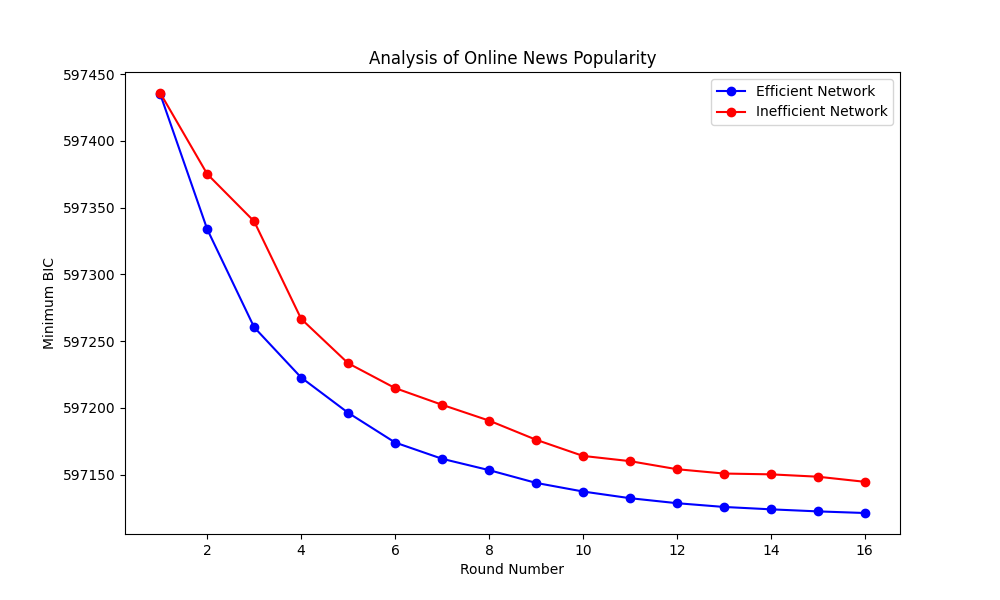
\includegraphics[scale=0.4]{figures/Online News Popularity Min.png}}
\centerline{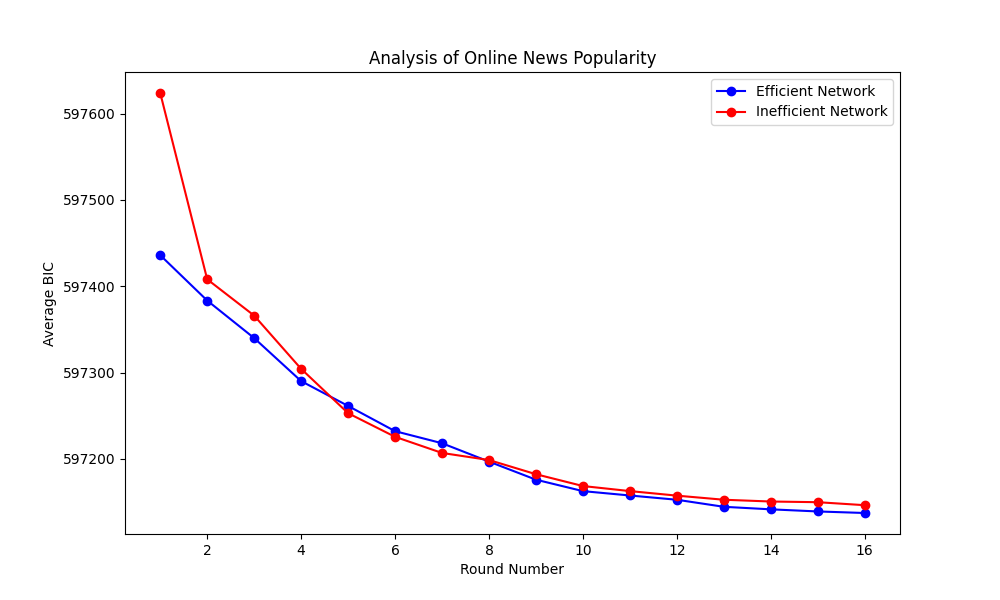
\includegraphics[scale=0.4]{figures/Online News Popularity Avg.png}}
\caption{Online News Popularity}
\label{fig}
\end{figure}

\begin{figure}[htbp]
\centerline{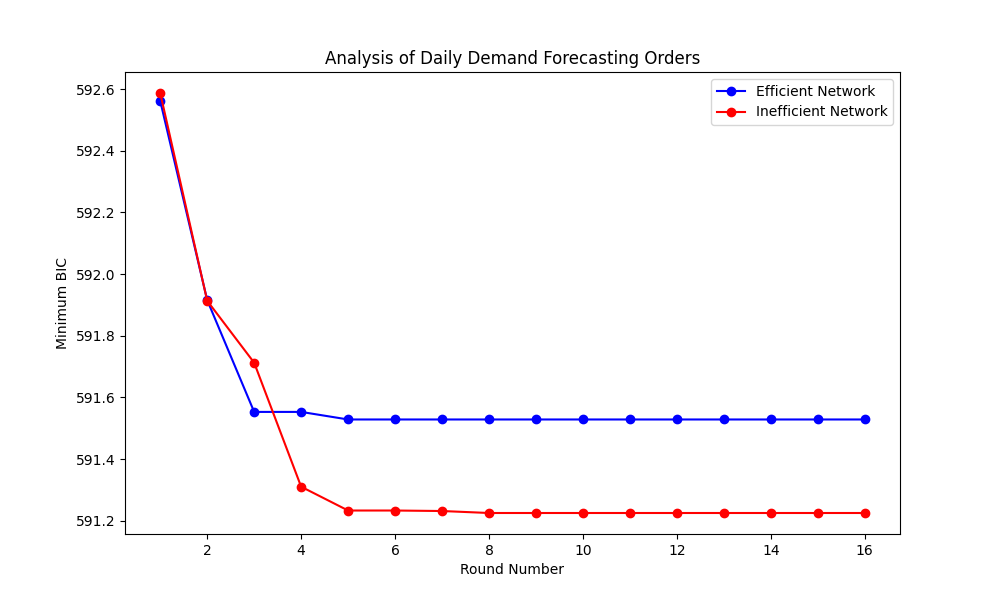
\includegraphics[scale=0.4]{figures/Daily Demand Forecasting Orders Min.png}}
\centerline{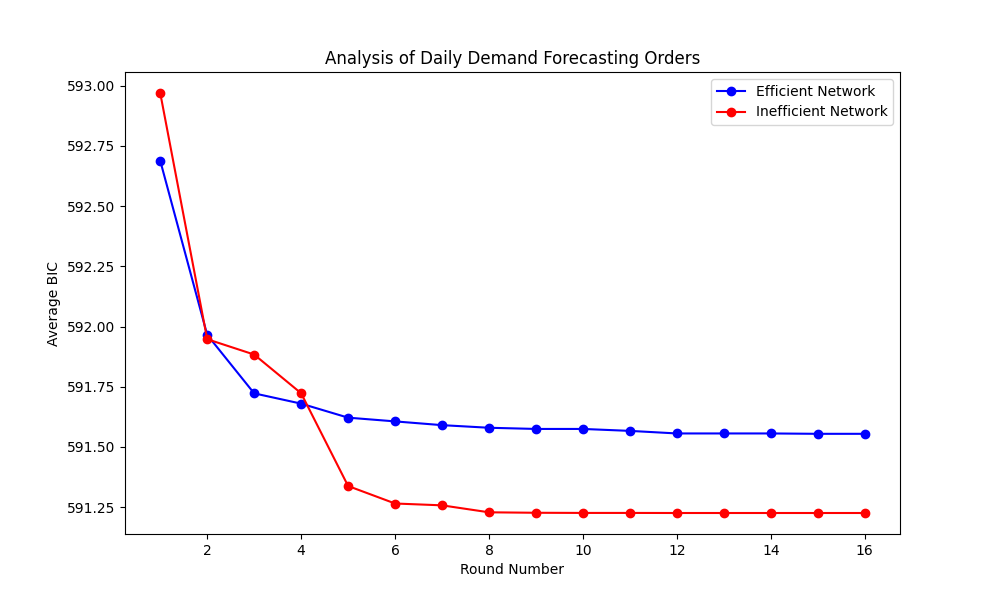
\includegraphics[scale=0.4]{figures/Daily Demand Forecasting Orders Avg.png}}
\caption{Daily Demand Forecasting Orders}
\label{fig}
\end{figure}

\section*{Acknowledgment}

I would like to thank Prof. Abhishek Samantray for their guidance, support, and encouragement throughout this research. Their expertise and insightful feedback were invaluable to the completion of this work.

\begin{thebibliography}{00}
\bibitem{b1} Brackbill, D. and Centola, D., 2020. Impact of network structure on collective learning: An experimental study in a data science competition. PLoS One, 15(9), p.e0237978.
\bibitem{b2} Mason, W. and Watts, D.J., 2012. Collaborative learning in networks. Proceedings of the National Academy of Sciences, 109(3), pp.764-769.
\bibitem{b3} Peters, L.D., Johnston, W.J., Pressey, A.D. and Kendrick, T., 2010. Collaboration and collective learning: networks as learning organizations. Journal of Business \& Industrial Marketing, 25(6), pp.478-484.
\bibitem{b4} Mason, W. and Watts, D., 2011. Collective problem solving in networks. Available at SSRN 1795224.
\bibitem{b5} Fang, C., Lee, J. and Schilling, M.A., 2010. Balancing exploration and exploitation through structural design: The isolation of subgroups and organizational learning. Organization Science, 21(3), pp.625-642.
\bibitem{b6} March, J.G., 1991. Exploration and exploitation in organizational learning. Organization science, 2(1), pp.71-87.
\bibitem{b7} Diehl, M. and Stroebe, W., 1987. Productivity loss in brainstorming groups: Toward the solution of a riddle. Journal of personality and social psychology, 53(3), p.497.
\bibitem{b8} Uzzi, B. and Spiro, J., 2005. Collaboration and creativity: The small world problem. American journal of Sociology, 111(2), pp.447-504.
\bibitem{b9} Balkundi, P. and Harrison, D.A., 2006. Ties, leaders, and time in teams: Strong inference about network structure’s effects on team viability and performance. Academy of Management journal, 49(1), pp.49-68.
\bibitem{b10} Reagans, R. and McEvily, B., 2003. Network structure and knowledge transfer: The effects of cohesion and range. Administrative science quarterly, 48(2), pp.240-267.
\end{thebibliography}

\end{document}
